\documentclass[12pt,fleqn,answers]{exam}
\usepackage{amssymb}
\usepackage[intlimits]{amsmath}
\usepackage{epsfig}
\usepackage{upgreek}
\usepackage[super]{nth}
\usepackage[colorlinks=true,linkcolor=black,anchorcolor=black,citecolor=black,filecolor=black,menucolor=black,runcolor=black,urlcolor=black]{hyperref}
\usepackage[letterpaper, margin=0.75in]{geometry}
\addpoints
\boxedpoints
\pointsinmargin
\pointname{pts}
\usepackage{tikz}
\usepackage{tkz-euclide}
\usetikzlibrary{shapes.geometric}
\usetikzlibrary{calc}
\usepackage[final]{microtype}
\frenchspacing
\usepackage[american]{babel}
\usepackage[T1]{fontenc}
\usepackage[upright]{fourier}
\usepackage{isomath}
\usepackage{upgreek,amsmath}
\usepackage{graphicx}

\newcommand{\dotprod}{\, {\scriptzcriptztyle\stackrel{\bullet}{{}}}\,}

\newcommand{\reals}{\mathbf{R}}
\newcommand{\lub}{\mathrm{lub}} 
\newcommand{\glb}{\mathrm{glb}} 
\newcommand{\complex}{\mathbf{C}}
\newcommand{\dom}{\mbox{dom}}
\newcommand{\range}{\mbox{range}}
\newcommand{\cover}{{\mathcal C}}
\newcommand{\integers}{\mathbf{Z}}
\newcommand{\vi}{\, \mathbf{i}}
\newcommand{\vj}{\, \mathbf{j}}
\newcommand{\vk}{\, \mathbf{k}}
\newcommand{\bi}{\, \mathbf{i}}
\newcommand{\bj}{\, \mathbf{j}}
\newcommand{\bk}{\, \mathbf{k}}
\DeclareMathOperator{\Arg}{\mathrm{Arg}}
\DeclareMathOperator{\Ln}{\mathrm{Ln}}
\newcommand{\imag}{\, \mathrm{i}}

\usepackage{graphicx}
\usepackage{color}
%\shadedsolutions
%\definecolor{SolutionColor}{rgb}{1,0.72,0.46} %{0.8,0.9,1}
\newcommand\AM{\textsc{am}}
\newcommand\PM{\textsc{pm}}
     
\newcommand{\quiz}{18}
\newcommand{\term}{Fall}
\newcommand{\due}{Tuesday 31 October 13:20}
\newcommand{\class}{MATH 202, Fall \the\year}
\begin{document}
%\large
\vspace{0.1in}
\noindent\makebox[3.0truein][l]{\textbf{\class}}
\textbf{Name:} \hrulefill \\
\noindent \makebox[3.0truein][l]{\textbf{In class work  \quiz}}
\textbf{Row and Seat}:\hrulefill\\

\normalsize
\noindent \emph{“The universe is a big place, perhaps the biggest.”} \hfill {\sc Kurt Vonnegut }

\vspace{0.1in}

\noindent  In class work  \textbf{\quiz}  has questions \textbf{1} 
through  \textbf{\numquestions} \/ with a total of 
\textbf{\numpoints\/} points. Turn in your work at the end of class 
\emph{on paper}. This assignment is due \emph{\due}.

\vspace{0.1in}



\begin{questions} 

\question The zero order Bessel function $J_0$ is defined by its power series.\footnote{This function is named in honor of Friedrich Bessel, a German 
 mathematician and scientist  who lived from 1784--1846. Bessel functions arise in  mechanical vibrations of a drum and electromagnetic
 waves in a coaxial cable, to mention just a few applications. }
 The power series is
\begin{equation*}
   J_0(x) = \sum_{k=0}^\infty  \frac{1}{(k \, !)^2}   \left(- \frac{x^2}{4} \right)^k 
               = 1 - \frac{x^2}{4} + \frac{x^4}{64} - \frac{x^6}{2304} +  \frac{x^8}{147456}  - \frac{{{x}^{10}}}{14745600} + \cdots     
 \end{equation*}
The radius  of convergence of this power series is infinity. 

\begin{parts}

\part [2] Find the numerical values of $J_0(0), J_0^\prime(0),$ and $ J_0^{\prime \prime}(0)$.


\begin{solution}[1.5in]  We have two representations for the the function $J_0$; one involves the 
summation and the other the ellipses (the $\dots$).  To find what we need, we only need to consider
the first few terms of the series, so let's do the calculation with just the first few terms.

Differentiating $J_0(x) = 1 - \frac{x^2}{4} + \frac{x^4}{64} - \frac{x^6}{2304} +  \frac{x^8}{147456}  - \frac{x^{10}} {14745600}$ termwise gives

\begin{align*}
J_0(x)   &= 1 - \frac{x^2}{4} + \frac{x^4}{64} - \frac{x^6}{2304} + \dots, \\
J_0^\prime(x)   &= - \frac{2 x }{4} + \frac{4 x^3}{64} - \frac{6 x^5}{2304} + \dots, \\
J_0^\prime(x)   &= - \frac{2 }{4} + \frac{4 \times 3 x^2}{64} - \frac{6  \times 5 x^4}{2304} + \dots, \\
\end{align*}
And evaluating at $x = 0$ yields
\begin{align*}
J_0(0)   &= 1, \\
J_0^\prime(0)   &= 0, \\
J_0^\prime(0)   &= - \frac{1}{2}.
\end{align*}

\end{solution}

\part [1] When $x$ has a modest magnitude, say $-10 < x < 10$, the summand $\frac{1}{(k \, !)^2}   \left(- \frac{x^2}{4}\right)^k$ 
converges to zero \emph{very quickly}. For example, when $x=10$ and $k=100$, the numeric value of the summand
is about $7.1  \times 10^{-177}$. So it's reasonable to conjecture that $J_0(x) \approx \sum_{k=0}^{100}  \frac{1}{(k \, !)^2}   \left(- \frac{x^2}{4} \right)^k $.  Use Desmos to graph $y = \sum_{k=0}^{100}  \frac{1}{(k \, !)^2}   \left(- \frac{x^2}{4} \right)^k$ for $-10 < x < 10$ and reproduce the graph here.

\begin{solution}
We'd need some theory to show that the graph is accurate--with a bit of faith, the graph is 

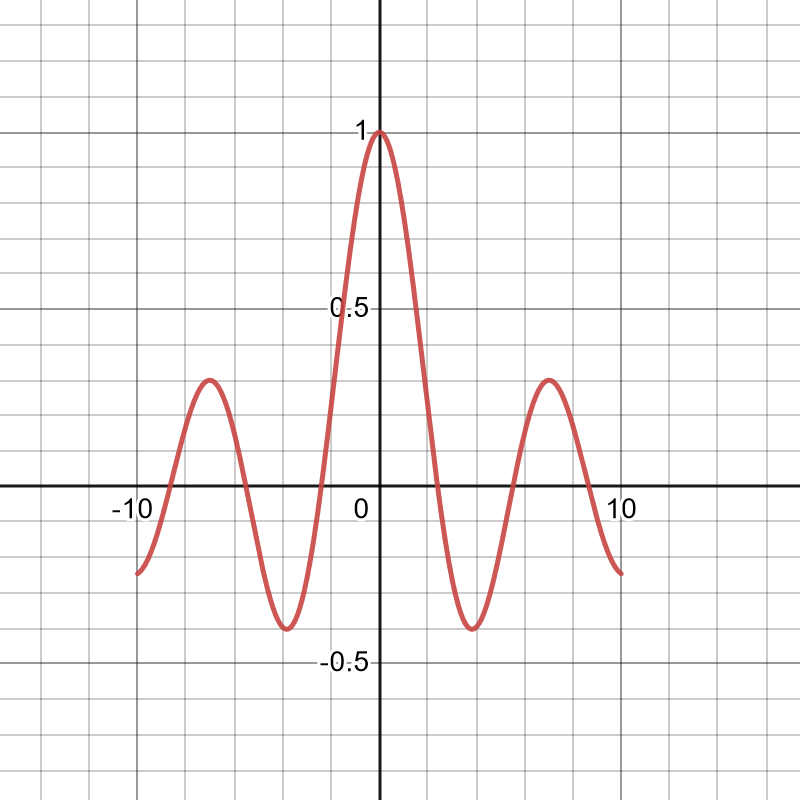
\includegraphics[scale=0.2]{desmos-graph(66).png}

\end{solution}

\end{parts}

%\newpage

\question A function $\mathcal{E}$ is defined by a power series; specifically $\displaystyle \mathcal{E}(x) = \sum_{k=0}^\infty \frac{1}{k!} x^k$.
The radius of convergence of this power series is infinity.


\begin{parts}

\part [1]  Find the numerical value of $\mathcal{E}(0)$.
\begin{solution}[0.5in]
\begin{equation*}
\mathcal{E}(0) = \sum_{k=0}^\infty \frac{1}{k!} 0^k = \sum_{k=0}^\infty \frac{1}{k!} \begin{cases} 1 & k =0 \\ 0 & k \neq 0 \end{cases} = 1.
\end{equation*}
\end{solution}


\part[1]  Find a power series for $\mathcal{E}^\prime$ and show that for  all real numbers $x$, we have $\mathcal{E}^\prime(x) = \mathcal{E}(x)$.


\begin{solution}[3.5in]
We have
\begin{equation*}
   \mathcal{E}^\prime(x) = \sum_{k=1}^\infty \frac{k}{k!} x^{k-1} \sum_{k=1}^\infty \frac{1}{(k-1)!} x^{k-1} 
   = \sum_{k=0}^\infty \frac{1}{k!} x^{k}  = \mathcal{E}(x).
\end{equation*}
\end{solution}




\part[1] The only solution to the initial value problem $\displaystyle \frac{\mathrm{d} y}{\mathrm{d} x} = y$ and $y \vert_{x=0} = 1$
is $y = \exp(x)$.  What is a simple formula for the function $\mathcal{E}$?

\begin{solution}
Since $\mathcal{E}^\prime = \mathcal{E}$ and $\mathcal{E}(0) = 1$, we've shown that $\mathcal{E} = \exp$.
\end{solution}
\end{parts}

\end{questions}
\end{document}
